\documentclass{beamer}
\usepackage{../tut-slides-LA}
\usepackage{../mathoperatorsLA}

\usepackage{amsmath,amssymb}
\usepackage{enumerate}
\usepackage[inline]{enumitem} 		%customize label
\newcommand{\labelitemi}{\raisebox{1pt}{\scalebox{.9}{$\blacktriangleright$}}}
\newcommand{\labelitemii}{$\vartriangleright$}
\newcommand{\labelitemiii}{--}

\usepackage[normalem]{ulem}
\usepackage{booktabs}
\usepackage{tcolorbox}
\newtcolorbox{highlightbox}{colback=cdblue!20,colframe=cddarkblue}

\usepackage{tabularx}
\usepackage{tabu}
\newcommand*\head{\rowfont{\bfseries}}
\newcommand*{\tw}{\rowfont{\ttfamily}}

\renewcommand{\tabularxcolumn}[1]{>{\hspace{0pt}}m{#1}}

\begin{document}	
	\title{Mathe 1 --- Lineare Algebra}
	\subtitle{Übung 1: Komplexe Zahlen }
	\author{Eric Kunze}
	\email{eric.kunze@mailbox.tu-dresden.de}
	\city{TU Dresden}
	\date{27. Oktober 2020}
%	\institute{Lehrstuhl für Grundlagen der Programmierung}
	\titlegraphic{
\includegraphics[width=2cm]{../TUD-white.pdf}}

	\maketitle
	
	\begin{frame} \frametitle{Wer bin ich?}
		\begin{minipage}{\dimexpr0.75\linewidth-\fboxrule-\fboxsep}
			\begin{itemize}
				\item \uline{Eric} [Kunze]
				\item \url{eric.kunze@mailbox.tu-dresden.de}
				\item Fragen, Wünsche, Vorschläge, \dots 
			\end{itemize}
		\end{minipage}
		\begin{minipage}{\dimexpr0.25\linewidth-\fboxrule-\fboxsep}
			
\includegraphics[width=3cm]{./tut01_pic.jpg}
		\end{minipage}		
	
	\begin{itemize}
		\item \textbf{Telegram:} \texttt{@oakoneric} bzw. \url{t.me/oakoneric}
	\end{itemize}
	\end{frame}

	\begin{frame} \frametitle{Einführung in die Mathematik für Informatiker}
			\begin{alertblock}{Teil A: Lineare Algebra}
				\begin{itemize}
					\item VL: Prof. Dr. Ulrike Baumann
					\item KA: Dr. Henri Mühle
					\item UE: me %\smiley				
				\end{itemize}
			\end{alertblock}
		
		\begin{block}{Teil B: Diskrete Strukturen}
			\begin{itemize}
				\item VL: Prof. Dr. Ellen Henke
				\item KA: Dr. Antje Noack
				\item UE: up to you
			\end{itemize}
		\end{block}
	\end{frame}

	\begin{frame}\frametitle{Einführung in die Mathematik für Informatiker}
		\textbf{Website für das Modul}: \\
		{\small \url{https://tu-dresden.de/mn/math/algebra/das-institut/beschaeftigte/antje-noack/dateien/einfmathinf} }
		
		\begin{center}
			\small
			\textit{ab hier: nur LAG-Teil (aber DIS ähnlich)}
		\end{center}
		
		
		\textbf{OPAL-Kurs}: \\
		{\small \url{https://bildungsportal.sachsen.de/opal/auth/RepositoryEntry/26113441794?0}}
		\begin{itemize}
			\item Informationen zur Lehrveranstaltung
			\item Skript zur Vorlesung
			\item Übungsblätter
			\item Hausaufgabenabgabe
			\item Lösungsvorschläge
			\item Forum
		\end{itemize}
	\end{frame}

	\begin{frame} \frametitle{Vorlesung vs. Übung}
		\centering
		\textbf{Was ist eine Übung?}
		
		''Lehrveranstaltung an der Hochschule, in der etw., bes. das Anwenden von Grundkenntnissen, von den Studierenden geübt wird`` [Duden]
		
		\pause
		
		\begin{tabularx}{\linewidth}{X|X}
			\hline
			\textbf{Vorlesung} & \textbf{Übung} \\ \hline \hline
			Vermittlung von neuem Wissen & Üben und Festigen des Stoffes der VL \\ \hline
			hohes Tempo & (selbst definierbares) langsameres Tempo \\ \hline
			wenig Interaktion & (sehr) viel Interaktion \\ \hline
			$\approx 50\%$ Verständnis & $>80\%$ Verständnis \\
			\hline
		\end{tabularx}
	\end{frame}

	\begin{frame} \frametitle{Was wird in der Übung erwartet?}
		\begin{itemize}
			\item Vorlesungsmaterial wurde vollständig angesehen
			\item Übungsblatt wurde angesehen (evtl. ausgedruckt, gespeichert, \dots)
			\item Aufgaben wurden \textit{im Vorfeld} vorbereitet
		\end{itemize}
	\end{frame}

	\begin{frame} \frametitle{Mein Material}
		
		\begin{block}{meine Website}
			\url{https://oakoneric.github.io}
		\end{block}
	
		\begin{itemize}[leftmargin=*]
			\item \url{https://github.com/oakoneric/lineare-algebra-ws20}
			\item \url{github.com} $\to$ oakoneric $\to$ lineare-algebra-ws20
			\medskip
			\item Slides und Beamer-Stuff
			\item evtl. zusätzliche Materialien (nach Bedarf)
			\item \alert{\textbf{kein Anspruch auf Vollständigkeit \& Korrektheit}}
			\item gefundene Fehler melden 
		\end{itemize}
	\end{frame}

%%%%%%%%%%%%%%%%%%%%%%%%%%%%%%%%%%%%%%%%%%%%%%%%%%%%%%%%%%%%%%%%%%%%%%%%%%%%%


\section{Übungsblatt 1}

\begin{frame} \frametitle{Komplexe Zahlen}
	\begin{equation*}
		\CC = \menge{a + b\i : a,b \in \R}
	\end{equation*}
Sei $z \in \CC$ eine beliebige komplexe Zahl. Wir können $z$ darstellen als $z = a + b\i$ mit reellen Zahlen $a,b \in \R$.
\begin{itemize}
	\item $\Re(z) \defeq a$ ist der \textbf{Realteil} von $z$
	\item $\Im(z) \defeq b$ ist der \textbf{Imaginärteil} von $z$ 
\end{itemize}

Wir können komplexe Zahlen u.a. addieren, subtrahieren, multiplizieren, dividieren und insbesondere
\begin{itemize}
	\item invertieren, d.h. $z^{-1}$ berechnen
	\item konjugieren, d.h. $\quer{z} \defeq a - b\i$ berechnen
\end{itemize}

\end{frame}


\begin{frame} \frametitle{Darstellung komplexer Zahlen}
%	\begin{equation*}
%		\CC = \menge{a + b \i : a,b \in \R}
%	\end{equation*}
	
%	\begin{minipage}{\dimexpr0.4\linewidth-\fboxrule-\fboxsep}
%		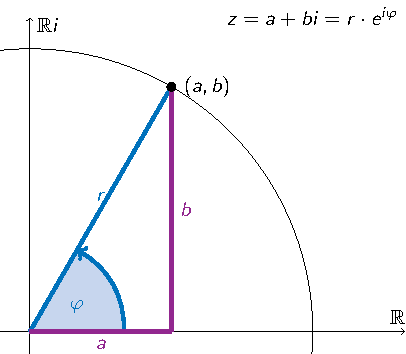
\includegraphics[width=\textwidth]{complex-plane}
%	\end{minipage}

%	\begin{minipage}{\dimexpr0.6\linewidth-\fboxrule-\fboxsep}
		Sei $z \in \CC$, $r = \abs{z}$ und $\phi = \Arg(z)$.
		\begin{itemize}
			\item $z = a + b \i$
			\item $z = r * \big( \cos(\phi) + \i \sin(\phi) \big)$
			\item $z = r * e^{\i \phi}$
		\end{itemize}
%\vspace{-0.5\baselineskip}
\begin{minipage}{\dimexpr0.6\linewidth-\fboxrule-\fboxsep}
	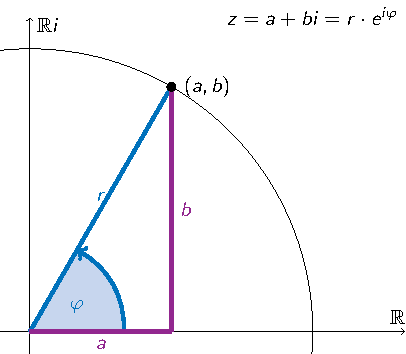
\includegraphics[width=\textwidth]{complex-plane}
\end{minipage}
\begin{minipage}{\dimexpr0.4\linewidth-\fboxrule-\fboxsep}
	\begin{align*}
		\cos(\phi) &= \frac{a}{r} \\
		\sin(\phi) &= \frac{b}{r}
	\end{align*}
\end{minipage}
	
\end{frame}






\section{Keine Angst vor Mathe!}

\begin{frame} \frametitle{Keine Angst vor Mathe!}
	\begin{block}{Euklid: Satz 4 in Buch II der ''Elemente``}
		Wird eine Strecke in zwei geteilt, dann ist das Quadrat über der ganzen Strecke gleich den Quadraten über den Teilen und dem doppelten Rechteck, das die Teile ergeben, zusammen.
	\end{block}


	\small siehe \url{http://www.opera-platonis.de/euklid/Buch2.pdf}
\end{frame}

\begin{frame} \frametitle{Keine Angst vor Mathe!}
	\begin{block}{al-Khwarizmi in Al-jabr wa'l muqabalah'}
		\small What must be the amount of a square, which, when twenty-one
		dirhems are added to it, becomes equal to the equivalent of ten
		roots of that square?
		
		\textbf{Solution}: Halve the number of the roots; the moiety is five.
		Multiply this by itself; the product is twenty-five. Subtract from
		this the twenty-one which are connected with the square; the
		remainder is four. Extract its root; it is two. Subtract this from
		the moiety of the root, which is five; the remainder is three. This
		is the root of the square which you required, and the square is
		nine. Or you may add the root of the moiety of the roots; the
		sum is seven; this is the root of the square which you sought for,
		and the square itself is forty nine.
	\end{block}
\end{frame}

\end{document}